\chapter{Разработка метода тактильного очувствления}\label{ch:ch4}


Четвертая глава раскрывает детали создания алгоритма построения карты с помощью тактильного очувствления, определения типа поверхности.

\section{Картографирование с помощью ощупывания поверхности}
Традиционно, карта для навигации представляется в виде облака точек. Тогда, без предложенного алгоритма, будут получено очень разреженное облако точек, где точки будут являться точками касания лапок робота с поверхностью.

Сделав предположение, что расстояние между ногами робота мало относительно целой пещеры, мы можем предположить, что поверхность между ногами является плоскостью.


В рамках исследования предполагается, что робот движется по поверхности, у которой каждому набору координат $x,\ y$ соответствует одно и только одно значение координаты $z$.

Был реализован следующий алгоритм. Вначале необходимо очистить оригинальное облако точек от шумов и усреднить близлежащие точки с помощью Voxel grid. Потом из него генерируется полигональная сетка с помощью 2D Триангуляции Делоне \pic{fig:delone_idea.png} (вогнутая оболочка \pic{fig:exp_concave_hull}). На ее основе получается необходимое плотное облако точек \pic{fig:sampled_pcd.png}. 

\begin{figure}[H]
    \centering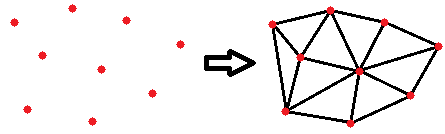
\includegraphics[height=5cm,width=1\textwidth,keepaspectratio]{delone_idea.png}
    \caption{2D Триангуляция Делоне (выпуклая оболочка)}
    \label{fig:delone_idea.png}
\end{figure}

Реализованный алгоритм проверялся, как в симуляции (Рис. \ref{fig:unsolvable_case}, \ref{fig:start_end_exp}), так и на реальном роботе \pic{fig:real_exp_map_creation}. Видео \quad \qrcode[height=1.5cm]{https://youtu.be/2dxHHTG4psQ}


\begin{figure}[H]
    \begin{subfigure}[t]{0.49\textwidth}
        \centering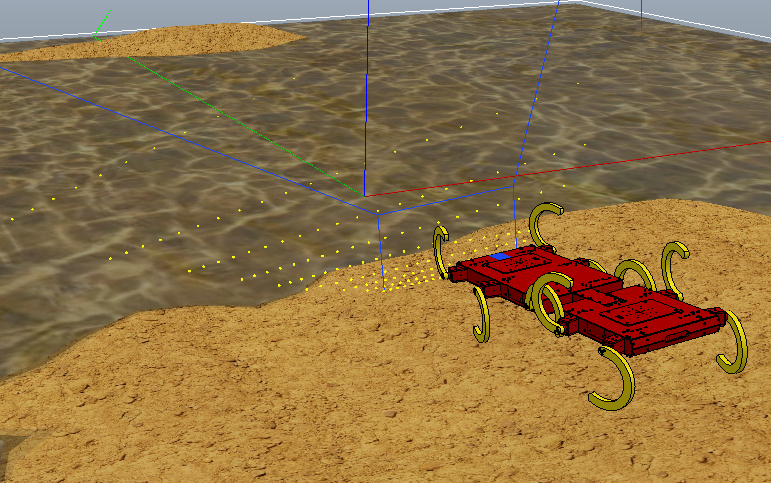
\includegraphics[height=5cm,width=1\textwidth,keepaspectratio]{terrain_w_water1.png}
        \caption{Начало движения}
    \end{subfigure}
    \begin{subfigure}[t]{0.49\textwidth}
        \centering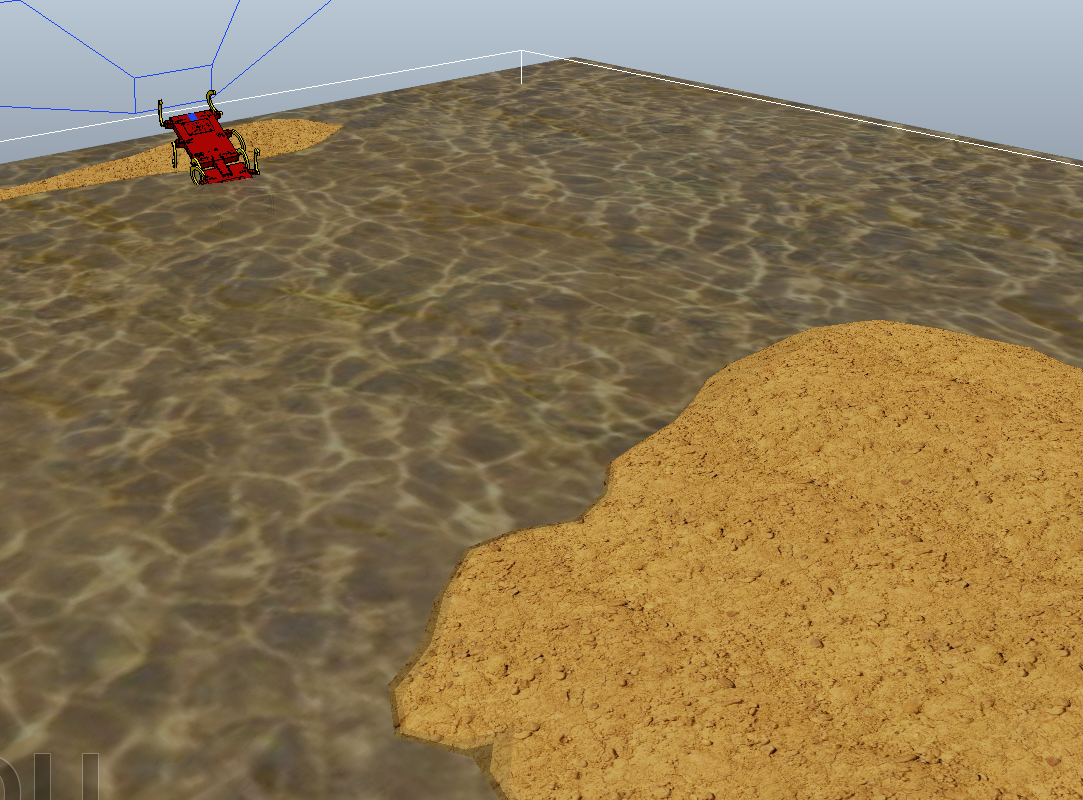
\includegraphics[height=5cm,width=1\textwidth,keepaspectratio]{terrain_w_water_end.png}
        \caption{Конец движения}
    \end{subfigure}
    \caption{Эксперимент в симуляторе}
    \label{fig:start_end_exp}
\end{figure}

Ниже представлены полученные результаты \pic{fig:result_meshes_blah}. Для оценки точности полученных данных использовались метрики C2C \eqref{eqn:hauff} и C2M \pic{fig:metrics}.

\begin{equation}
    \label{eqn:hauff}
    d_{H}(X,\;Y)=\sup _{m\in M}\left\{\,|\mathrm {dist} _{X}(m)-\mathrm {dist} _{Y}(m)|\,\right\}    
\end{equation}
Где \nom{$X,\ Y$}{непустые подмножества метрического пространства $M$}; \nom{$\mathrm {dist} _{X}\colon M\to \mathbb {R}$}{обозначает функцию расстояния до множества $X$}.



\begin{figure}[h]
    \begin{center}
    \begin{subfigure}[t]{0.4\textwidth}
        \centering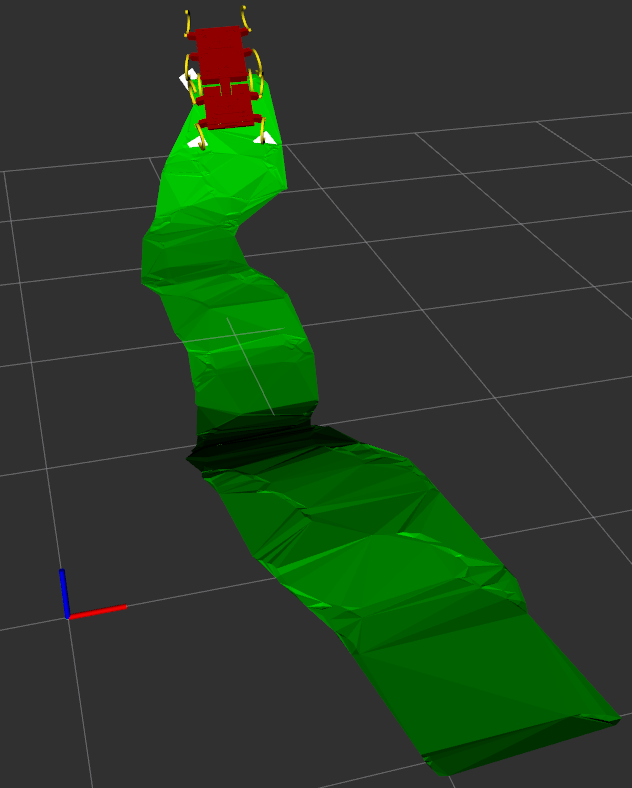
\includegraphics[height=8cm,width=1\textwidth,keepaspectratio]{mesh_rviz.png}
        \caption{Полигональная сетка, созданная 2D Триангуляцией Делоне (вогнутая оболочка)}
    \end{subfigure}
    \begin{subfigure}[t]{0.59\textwidth}
        \centering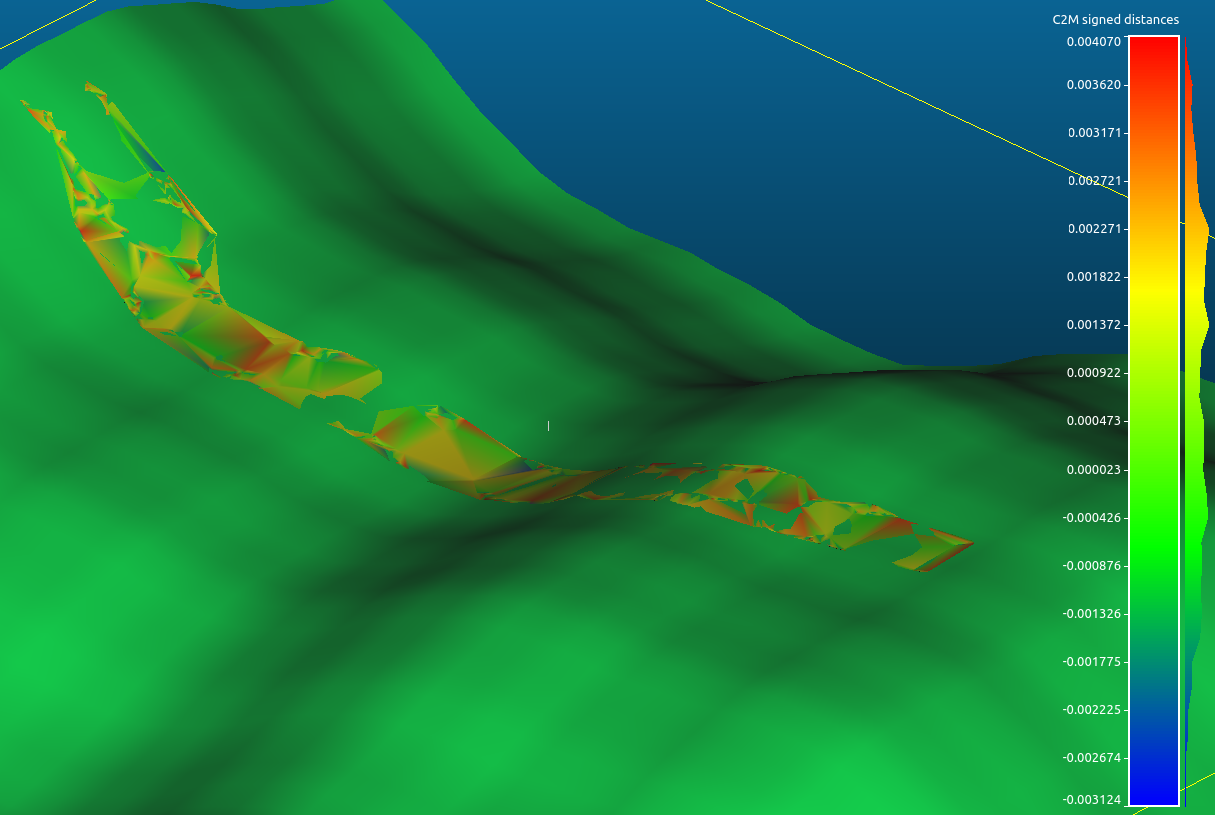
\includegraphics[height=8cm,width=1\textwidth,keepaspectratio]{mesh_comp.png}
        \caption{Наложенные полигональные сетки}
    \end{subfigure}

    \begin{subfigure}[t]{0.9\textwidth}
            \centering
             \begin{tikzpicture}
                % Include the image in a node
                \node [above right, inner sep=0] (image) at (0,0) 
                {\centering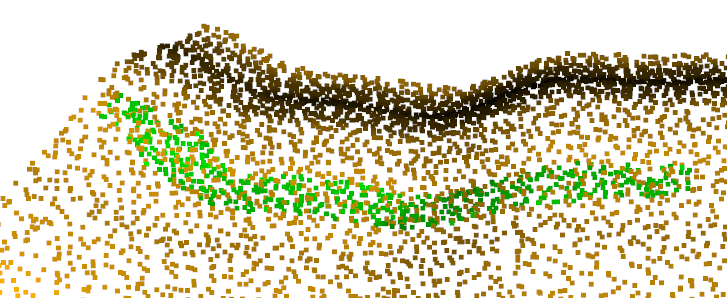
\includegraphics[height=8cm,width=1\textwidth,keepaspectratio]{sampled_pcd.png}};          
                % Create scope with normalized axes
                \begin{scope}[
                    x={($ 0.1*(image.south east)$)},
                    y={($ 0.1*(image.north west)$)}]
                    \draw[stealth-, very thick,green] (3,8) -- (2,8.5);
                    \draw[stealth-, very thick,green] (1,5.5) -- (2,8.5)
                    node[rounded corners=3pt,above,black,fill=white]{\tiny Ground Truth Point Cloud};
         
                    \draw[stealth-, very thick,green] (5.5,3) -- (5.5,8.5)
                    node[rounded corners=3pt,above,black,fill=white]{\tiny Generated Point Cloud};
                \end{scope}
            \end{tikzpicture}
            \caption{Наложенные облака точек}
            \label{fig:sampled_pcd.png}
    \end{subfigure}
    \caption{Результат эксперимента}
    \label{fig:result_meshes_blah}
\end{center}
\end{figure}

\begin{figure}[h]
    \begin{subfigure}{0.9\textwidth}
        \centering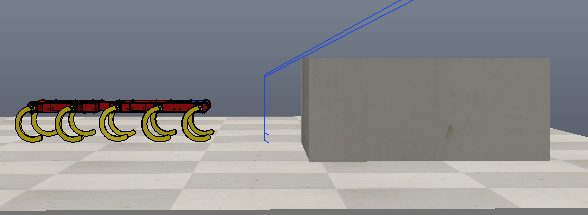
\includegraphics[height=8cm,width=1\textwidth,keepaspectratio]{postament_orig.png}
        \caption{Результат эксперимента по построению карты постамента, симулятор}
        \label{fig:postament_orig.png}
    \end{subfigure}
    \begin{subfigure}{0.9\textwidth}
        \centering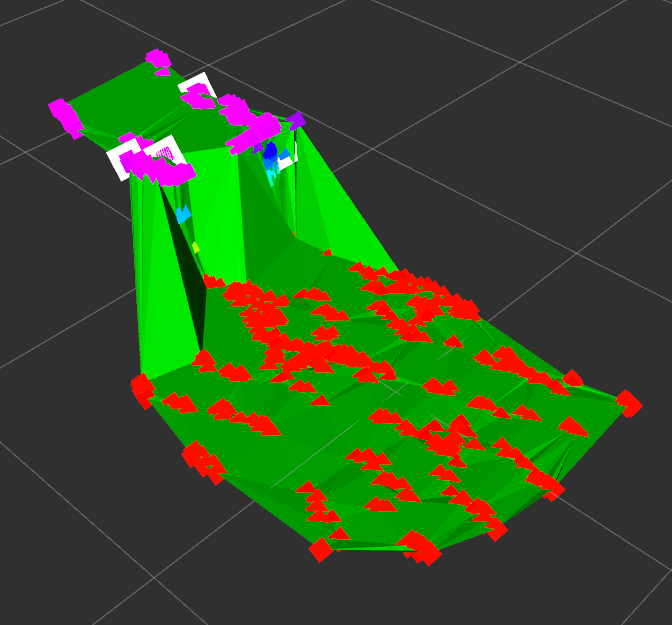
\includegraphics[height=8cm,width=1\textwidth,keepaspectratio]{postament_mesh.png}
        \caption{Результат эксперимента по построению карты постамента, Rviz, полигональная сетка}
        \label{fig:postament_mesh.png}
    \end{subfigure}

\caption{Результат эксперимента по построению карты постамента}
\label{fig:}
\end{figure}

На рисунке \ref{fig:exp_concave_hull} проиллюстрирована  важность модификации триангуляции Делоне. Как можно заметить \pic{fig:conv_convex.png} алгоритм построил карту местности там, где робот не ходил и стоит стена. При использовании вогнутой оболочки \pic{fig:conv_concave.png} данная проблема не наблюдается.

\begin{figure}[h]
    \begin{subfigure}[t]{0.3\textwidth}
        \centering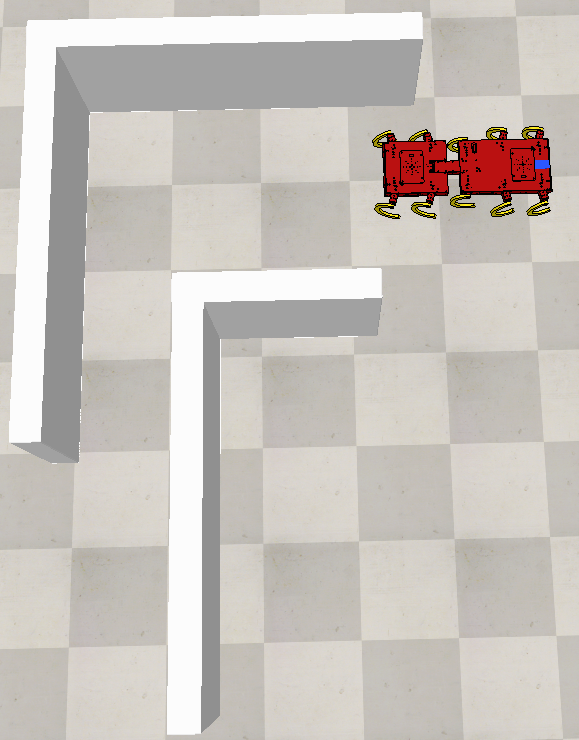
\includegraphics[height=8cm,width=1\textwidth,keepaspectratio]{convex_terr.png}
        \caption{Пример поля}
        \label{fig:convex_terr.png}
    \end{subfigure}
    \hfill
    \begin{subfigure}[t]{0.33\textwidth}
            \centering
             \begin{tikzpicture}
                % Include the image in a node
                \node [above right, inner sep=0] (image) at (0,0) 
                {\centering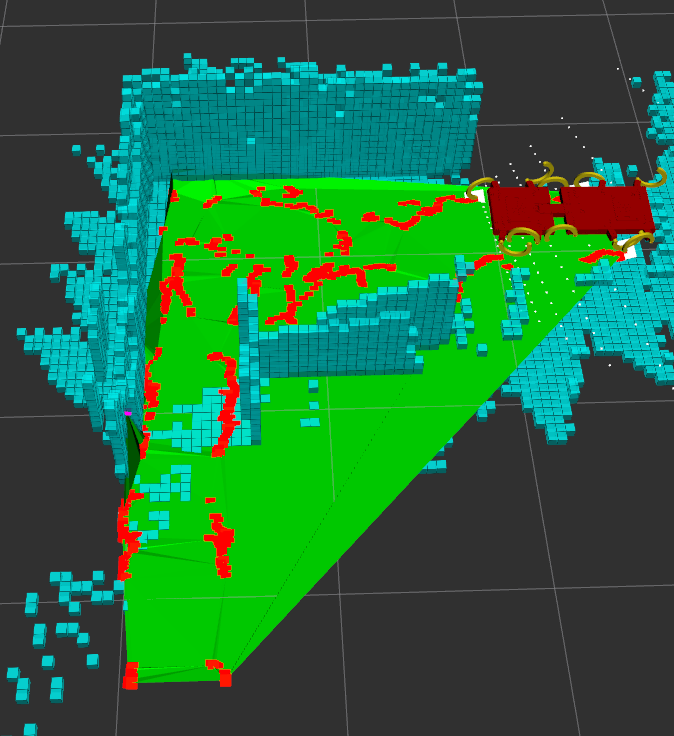
\includegraphics[height=8cm,width=1\textwidth,keepaspectratio]{conv_convex.png}};          
                % Create scope with normalized axes
                \begin{scope}[
                    x={($ 0.1*(image.south east)$)},
                    y={($ 0.1*(image.north west)$)}]
                    \draw[stealth-, very thick,green] (5.2,3.5) -- ++(1,-1)
                    node[rounded corners=3pt,right,black,fill=white]{\tiny Generated mesh};
                    
                    \draw[stealth-, very thick,green] (5.5,5.5) -- (7.4,4)
                    node[rounded corners=3pt,right,black,fill=white]{\tiny Lidar data};
                    \draw[stealth-, very thick,green] (3.4,0.8) -- (5,1);            
                    \draw[stealth-, very thick,green] (3.4,2.6) -- (5,1)
                    node[rounded corners=3pt,right,black,fill=white]{\tiny Cloud of contact points};
                \end{scope}
            \end{tikzpicture}
            \caption{Выпуклая оболочка}
            \label{fig:conv_convex.png}
    \end{subfigure}
    \hfill
    \begin{subfigure}[t]{0.30\textwidth}
        \centering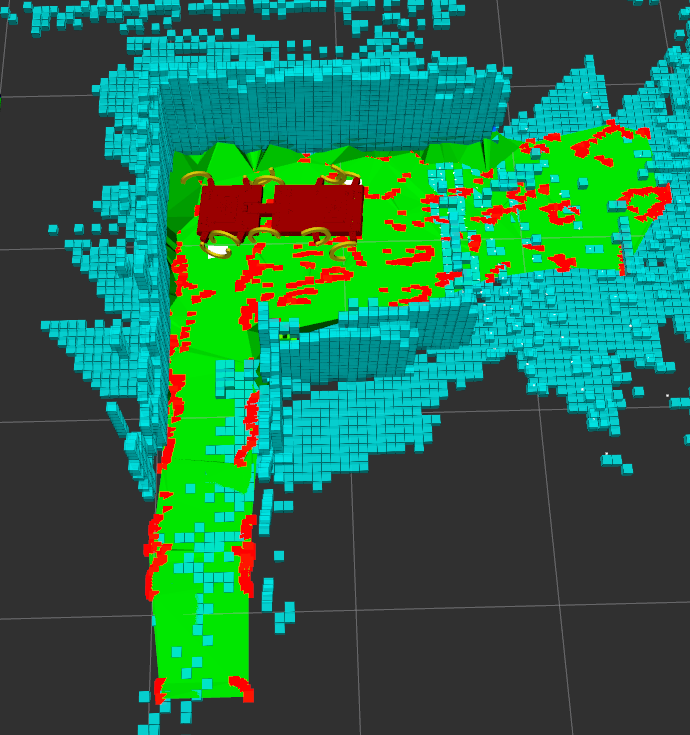
\includegraphics[height=8cm,width=1\textwidth,keepaspectratio]{conv_concave.png}
        \caption{Вогнутая оболочка}
        \label{fig:conv_concave.png}
    \end{subfigure}
    \caption{Объяснение необходимости модификации алгоритма Делоне}
    \label{fig:exp_concave_hull}
\end{figure}

\begin{figure}[h]
    \begin{subfigure}[t]{0.49\textwidth}
        \centering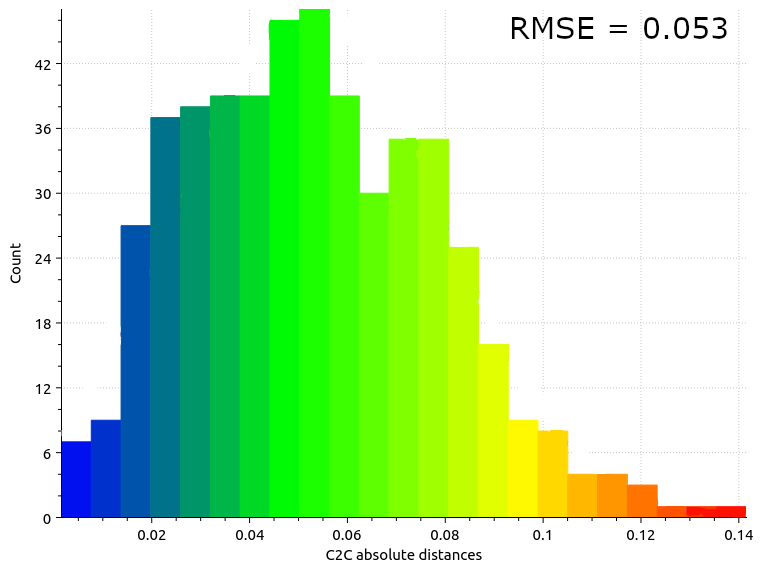
\includegraphics[height=8cm,width=1\textwidth,keepaspectratio]{pcd_hist.png}
        \caption{Метрика C2C: гистограмма ошибок (абсолютное расстояние от точки до ближайшей реферальной точки)}
        \label{fig:metric_c2c}
    \end{subfigure}
    \begin{subfigure}[t]{0.49\textwidth}
        \centering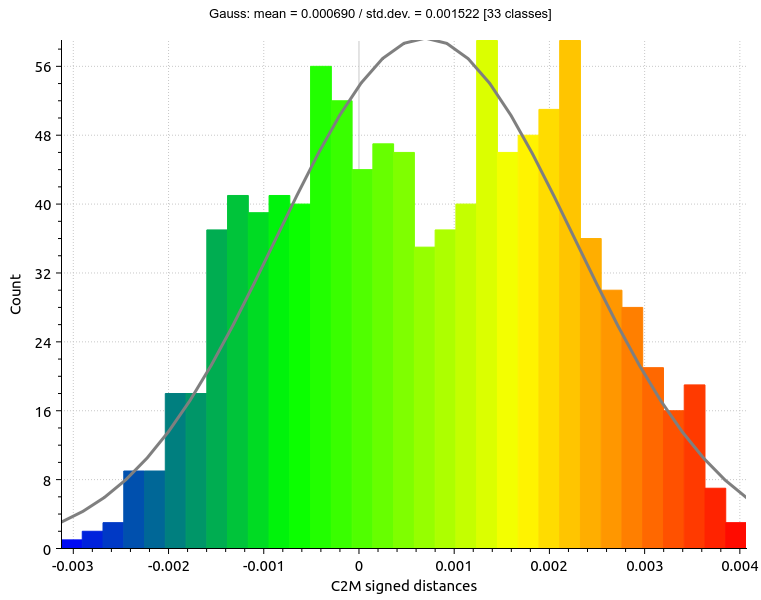
\includegraphics[height=8cm,width=1\textwidth,keepaspectratio]{mesh_hist.png}
        \caption{Метрика C2M: Гистограмма ошибок (относительное расстояние от точки до ближайшей реферальной точки)}
        \label{fig:metric_c2m}
    \end{subfigure}
    \caption{Метрики оценки точности полученной карты}
    \label{fig:metrics}
\end{figure}


\begin{figure}[h]
    \begin{subfigure}[t]{0.49\textwidth}
            \centering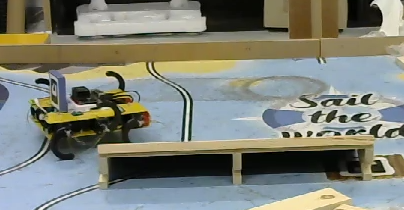
\includegraphics[height=8cm,width=1\textwidth,keepaspectratio]{real_robot_mesh_video_preview.png}
        \caption{Робот проходит препятствие}
        \label{fig:real_robot_mesh_video_preview.png}
    \end{subfigure}
    \begin{subfigure}[t]{0.49\textwidth}
        \centering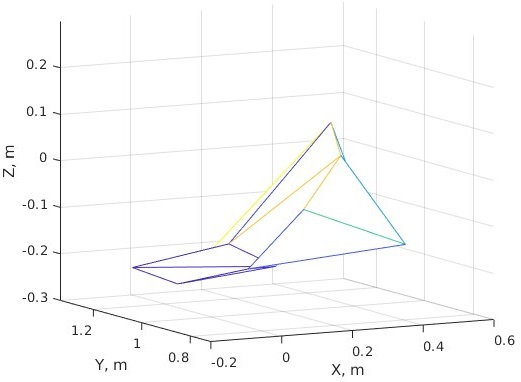
\includegraphics[height=8cm,width=1\textwidth,keepaspectratio]{real_mesh.jpg}
        \caption{Полученная полигональная сетка}
        \label{fig:real_mesh.jpg}
    \end{subfigure}
    \caption{Пример натурного эксперимента}
    \label{fig:real_exp_map_creation}
\end{figure}

Как итог, среднеквадратичная ошибка для C2C метрики была в среднем равна 5 см. А для C2M 1 см. В натурном эксперименте среднеквадратичная ошибка по метрике C2C получился 8 см.

\section{Определение типа поверхности}

Задачу определения типа поверхности можно определить следующим образом. Робот идет по поверхности, и собирает данные с датчиков силы, с момента на моторе и IMU. На основе предварительного обучения, данные обрабатываются и кластеризуются, на основе предварительно определенной базе знаний территорий.

Задачу обучения удобнее всего проводить в лабораторных условиях. Экспериментальная установка соответствует следующим требованиям: возможность установить новые поверхность и сменять их быстро. Это нужно для легкого создания базы знаний поверхностей. Бесконечное движение, для скорости обучения. Узел с ногой должен быть взят с робота, чтобы не пришлось решать похожую задачу на роботе.

Все это было достигнуто благодаря разборному экспериментальному столу и 2ух степенному механизму, который ходит по окружности \pic{fig:s_shape_leg/s_leg_setup.JPG}. Для бесконечного движения пришлось соединить две ноги робота в одну. На рисунке ниже \pic{fig:s_shape_leg/leg_design.png} показаны как установлены сенсоры на получившейся ноге.

\begin{figure}[H]
    \begin{subfigure}[t]{0.48\textwidth}
        \centering
        \begin{tikzpicture}
            % Include the image in a node
            \node [above right, inner sep=0] (image) at (0,0)
            {\centering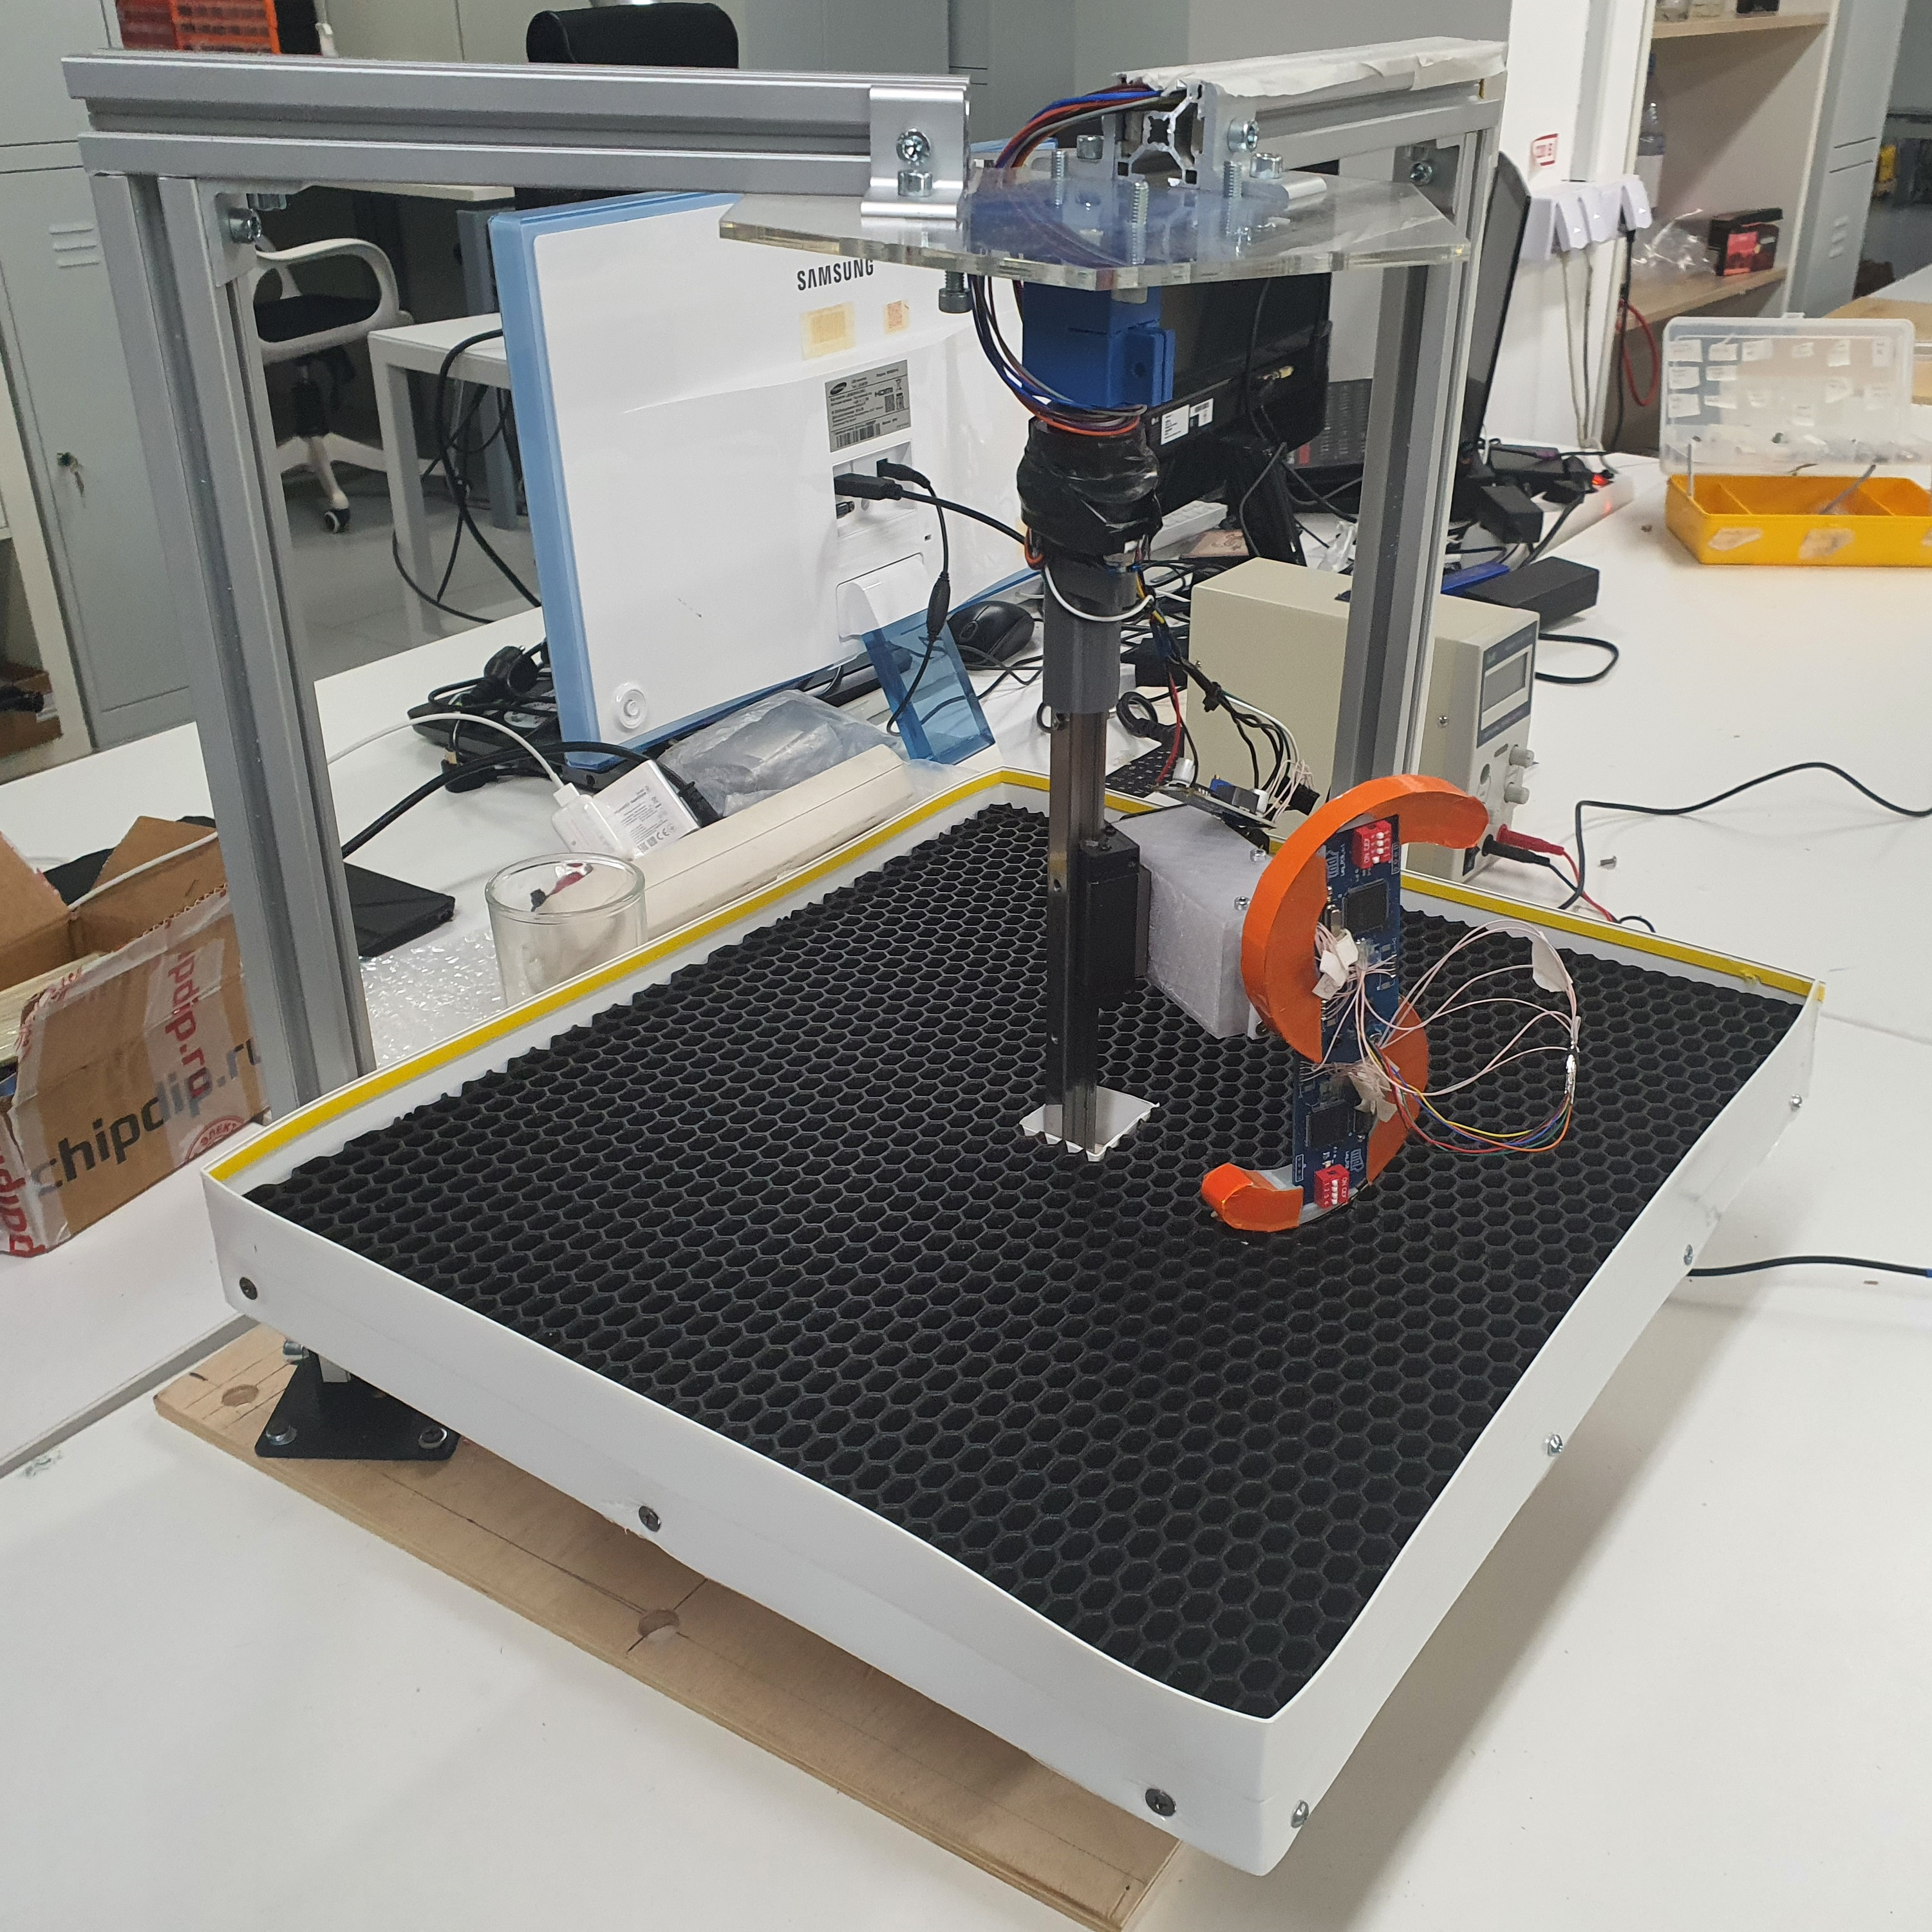
\includegraphics[height=8cm,width=1\textwidth,keepaspectratio]{s_shape_leg/s_leg_setup.JPG}};
            % Create scope with normalized axes
            \begin{scope}[
                    x={($ 0.1*(image.south east)$)},
                    y={($ 0.1*(image.north west)$)}]
                \draw[stealth-, very thick,green] (3.5,2.5) -- (3,1.5)
                node[rounded corners=3pt,below,black,fill=white]{\tiny Table for surfaces};

                \draw[stealth-, very thick,green] (7.1,5.4) -- (7.4,7)
                node[rounded corners=3pt,above right,black,fill=white]{\tiny Self-made PCB};

                \draw[very thick,green] (6,6.1) rectangle (8.5,3.5)
                node[above left,black,fill=green]{\tiny S leg};
            \end{scope}
        \end{tikzpicture}
        \caption{Общий вид экспериментальной установки}
        \label{fig:s_shape_leg/s_leg_setup.JPG}
    \end{subfigure}
    \begin{subfigure}[t]{0.24\textwidth}
        \centering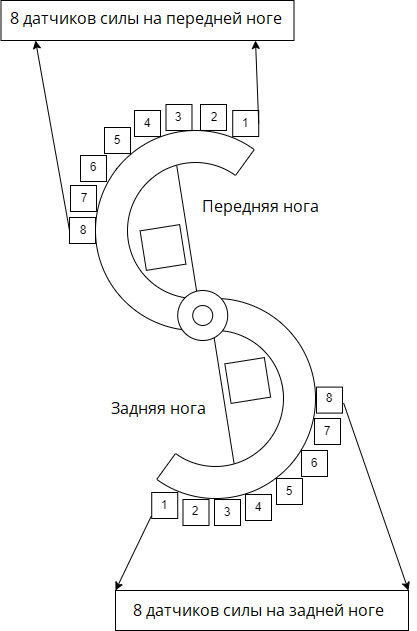
\includegraphics[height=8cm,width=1\textwidth,keepaspectratio]{s_shape_leg/leg_design.png}
        \caption{Пояснение по расположению сенсоров на ноге робота}
        \label{fig:s_shape_leg/leg_design.png}
    \end{subfigure}
    \begin{subfigure}[t]{0.24\textwidth}
        \centering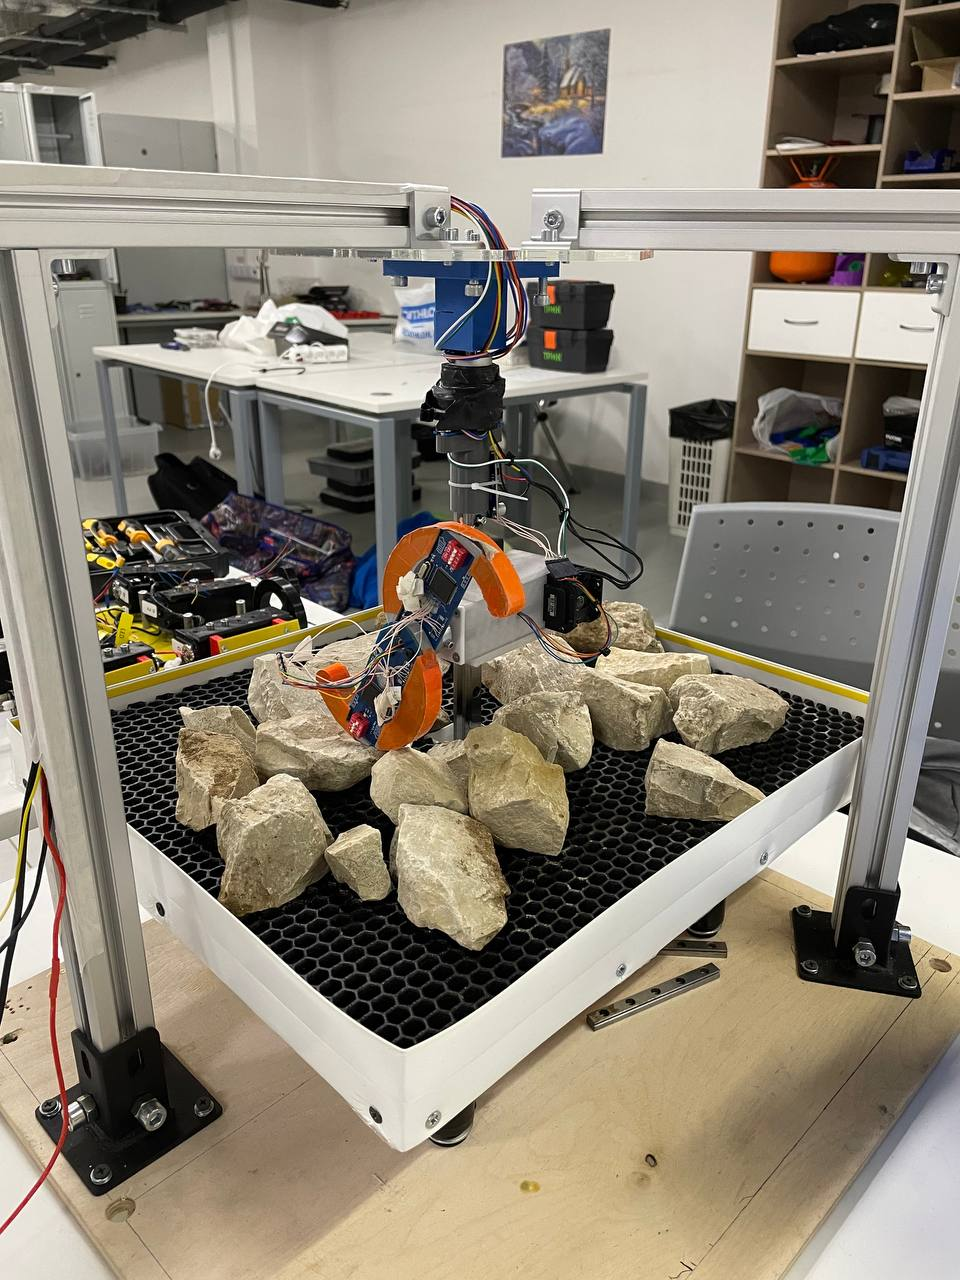
\includegraphics[height=8cm,width=1\textwidth,keepaspectratio]{s_shape_leg/view.jpg}
        \caption{Каменистая поверхность}
        \label{fig:s_shape_leg/view.jpg}
    \end{subfigure}
    \caption{Экспериментальная установка для определения типа поверхности}
\end{figure}

Были взяты 2 сильно разных поверхности и изучены сырые данные. Резина \pic{fig:s_shape_leg/s_leg_setup.JPG}  \quad \qrcode[height=1.5cm]{https://gifyu.com/image/SxatY} \quad, камень \pic{fig:s_shape_leg/view.jpg} \quad \qrcode[height=1.5cm]{https://gifyu.com/image/Sxatt} 

% \begin{figure}[H]
%     \begin{subfigure}[t]{0.49\textwidth}
%         \centering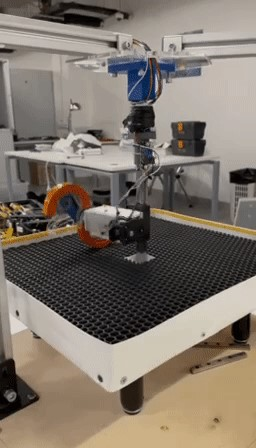
\includegraphics[height=4cm,width=1\textwidth,keepaspectratio]{s_shape_leg/flat.jpg}
%         \caption{Резина}
%         \label{fig:s_shape_leg/flat.jpg}
%     \end{subfigure}
%     \hfill
%     \begin{subfigure}[t]{0.49\textwidth}
%         \centering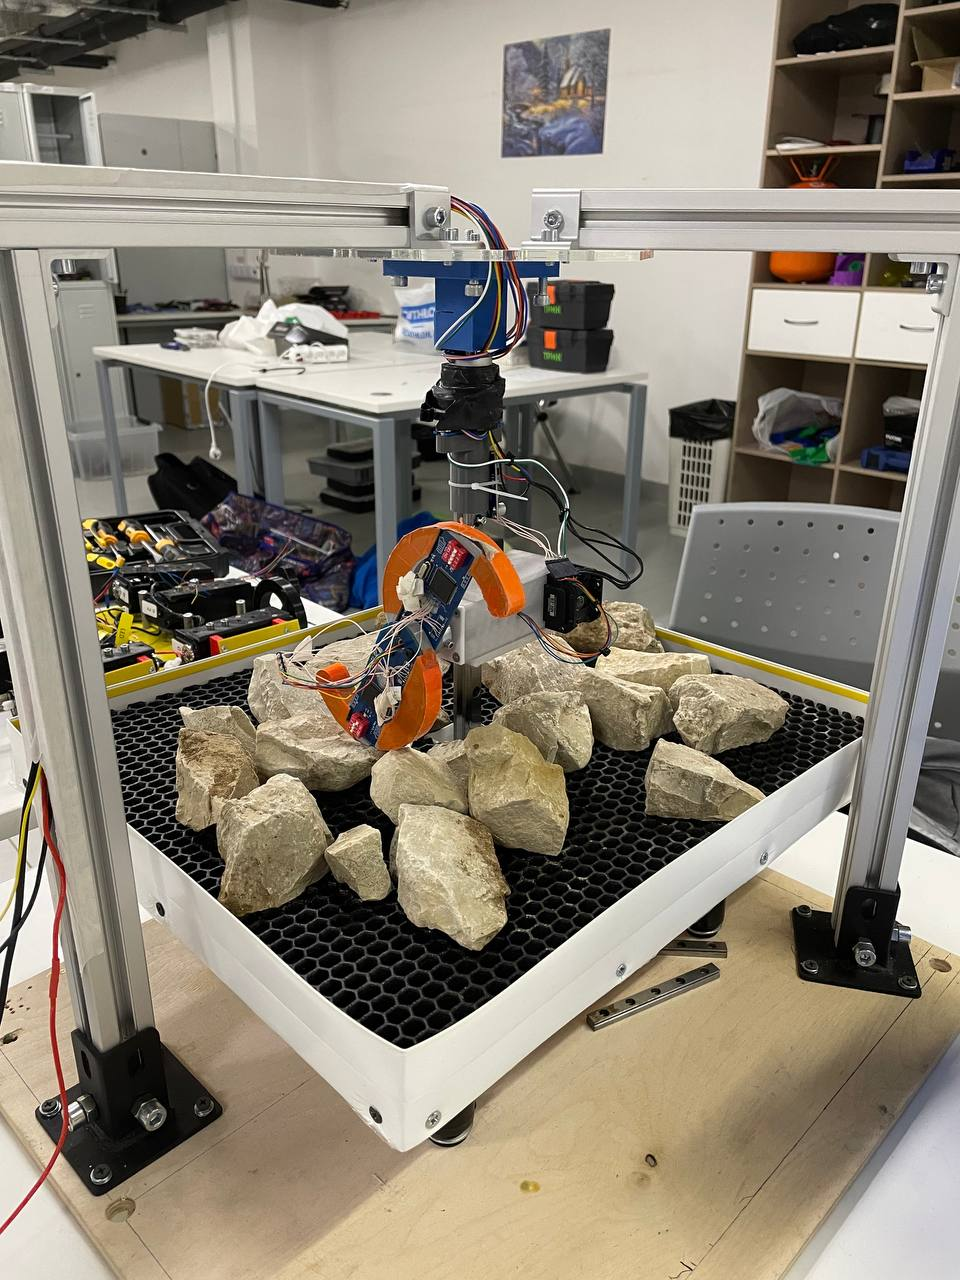
\includegraphics[height=4cm,width=1\textwidth,keepaspectratio]{s_shape_leg/view.jpg}
%         \caption{Каменистая поверхность}
%         \label{fig:s_shape_leg/view.jpg}
%     \end{subfigure}
%     \caption{Типы определяемых поверхностей}
% \end{figure}

Ниже \pic{fig:data_from_legs} представлены сырые данные с лапок робота. Сырые данные легко различить, но можно заметить, что абсолютные значения у разных сегментов различно. Поэтому при обучении необходимо их нормализовать.

\begin{figure}[H]
    \begin{subfigure}[t]{0.9\textwidth}
        \centering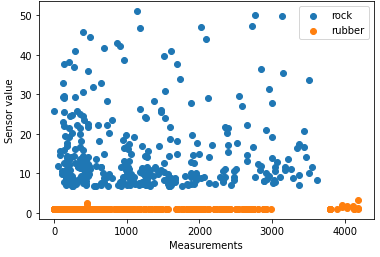
\includegraphics[height=8cm,width=1\textwidth,keepaspectratio]{s_shape_leg/segment8_compare_front.png}
        \caption{Передняя часть ноги, 8ой сегмент}
    \end{subfigure}

    \begin{subfigure}[t]{0.9\textwidth}
        \centering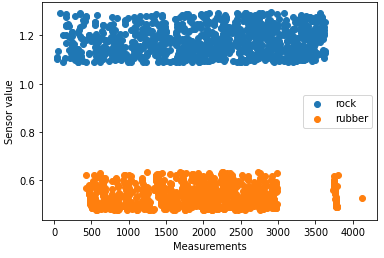
\includegraphics[height=8cm,width=1\textwidth,keepaspectratio]{s_shape_leg/segment6_compare_front.png}
        \caption{Передняя часть ноги, 6ой сегмент}
    \end{subfigure}
    \caption{Сравнение сырых данных после эксперимента с разных сегментов ноги}
    \label{fig:data_from_legs}
\end{figure}

\begin{figure}[H]
    \centering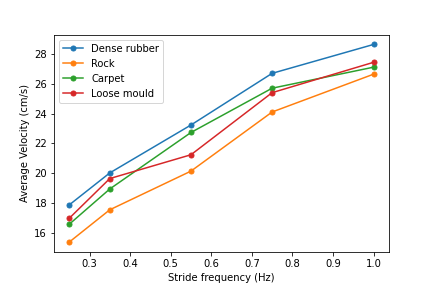
\includegraphics[height=8cm,width=1\textwidth,keepaspectratio]{s_shape_leg/AverageVelocity (1).png}
    \caption{Средняя линейная скорость робота}
    \label{fig:s_shape_leg/AverageVelocity (1).png}
\end{figure}

\begin{figure}[H]
    \centering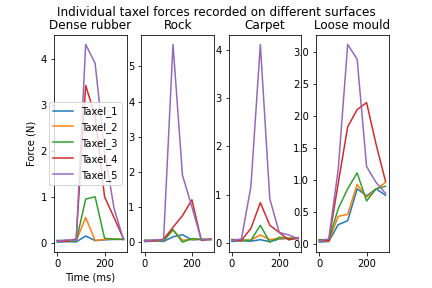
\includegraphics[height=8cm,width=1\textwidth,keepaspectratio]{s_shape_leg/TaxelIndForce_full.png}
    \caption{Запись активных такселей на разных поверхностях}
    \label{fig:s_shape_leg/TaxelIndForce_full.png}
\end{figure}

Карта местности может быть построена с помощью 2D триангуляции Делоне (вогнутая оболочка). Входными данными для алгоритма является разреженное облако точек касаний робота поверхности. Они получены с помощью преобразователя силы на основе Velostat.

Точность, полученная в симуляторе равна примерно 5 см, а во время натурного эксперимента -- 8 см, что является адекватным результатом для поставленной задачи.

С помощью разработанного преобразователя силы возможно различать 2 типа поверхности: резину и каменистую гряду.